% ===== Part A: 원문 PDF 1–10쪽 (제목, 초록, 1장, 2장 도입, 2.1, 2.2) =====
\begin{center}
{\LARGE 유한 부호 길이 정보이론\par}
\vspace{0.4em}
{\large Finite-Blocklength Information Theory\par}
\vspace{1.2em}
Junyuan Gao\textsuperscript{a,b}, Shuao Chen\textsuperscript{b}, Yongpeng Wu\textsuperscript{b,$*$}, Liang Liu\textsuperscript{a}, Giuseppe Caire\textsuperscript{c}, H. Vincent Poor\textsuperscript{d}, Wenjun Zhang\textsuperscript{b}\par
\vspace{0.8em}
{\small\itshape
\textsuperscript{a}Department of Electrical and Electronic Engineering, The Hong Kong Polytechnic University, Hong Kong SAR, China\par
\textsuperscript{b}Department of Electronic Engineering, Shanghai Jiao Tong University, Shanghai, Minhang 200240, China\par
\textsuperscript{c}Communications and Information Theory Group, Technische Universität Berlin, Berlin, 10587, Germany\par
\textsuperscript{d}Department of Electrical and Computer Engineering, Princeton University, Princeton, NJ 08544, USA\par}
\vspace{0.6em}
{\small \textsuperscript{$*$}교신저자. 이메일: \texttt{yongpeng.wu@sjtu.edu.cn} (Yongpeng Wu)\par}
\end{center}

\begin{quote}
\textbf{초록}\par
무선 통신 시스템의 근본 한계(fundamental limit)를 다루는 전통적인 점근(asymptotic) 정보이론 연구는 주로 몇 가지 이상적인 가정에 기대어 왔다. 부호 길이(blocklength)가 무한하고 오류 확률이 0으로 사라진다는 가정이 대표적이다. 이러한 가정 덕분에 수학적으로 다루기 쉬운(tractable) 결과를 얻을 수 있지만, 새로 등장하는 차세대 무선 응용의 엄격한 요구 조건은 담아내지 못한다. 초고신뢰 저지연 통신(ultra-reliable low latency communication)이나 초대규모 기계형 통신(ultra-massive machine type communication) 같은 응용은 짧은 패킷 통신(short-packet communication), 극히 낮은 지연, 낮은 에너지 소비 등 훨씬 폭넓은 특성을 지원해야 한다. 이런 응용을 더 잘 뒷받침하려면 유한 부호 길이(finite blocklength) 정보이론을 고려해야 한다. 이 논문은 이 분야의 진전을 포괄적으로 살펴본 뒤 미해결 문제를 논의한다. 구체적으로, 먼저 비점근(non-asymptotic) 영역에서 원천 부호화(source coding)의 근본 한계를 다룬다. 이때 점대점(P2P, point-to-point) 및 다중 단말(multiterminal) 환경의 무손실 압축(lossless compression)과 손실 압축(lossy compression)에 특히 초점을 맞춘다. 이어서 P2P 채널, 다중 접속 채널(multiple access channel), 새로 떠오르는 대규모 접속 채널에서 채널 부호화(channel coding)의 근본 한계를 논의한다. 나아가 결합 원천-채널 부호화(joint source and channel coding)의 최근 진전을 소개하고, 비점근 영역에서 이 방식이 분리 원천-채널 부호화(separate source and channel coding)보다 성능 면에서 상당히 앞선다는 점을 부각한다. 각 부분에서는 다양한 비점근 달성 가능성 한계(achievability bound), 역 한계(converse bound), 근사(approximation)와 그 밑바탕의 핵심 아이디어를 검토한다. 이러한 한계와 근사는 미래 무선 통신 시스템 설계에 공학적 통찰(insight)을 주는 데 꼭 필요하다.

\medskip
\textit{주제어:} 근사, 유한 부호 길이 정보이론, 저지연, 비점근 한계, 원천 및 채널 부호화
\end{quote}

\section{서론}

초고신뢰 저지연 통신(URLLC, ultra-reliable low latency communications)은 5세대(5G) 무선 네트워크의 3대 주요 사용 사례 가운데 하나이다. URLLC는 종단 간 지연과 신뢰도에 대한 요구가 엄격한 핵심 응용의 토대가 된다 [1]. 산업 자동화, 자율 주행, 원격 의료, 증강 현실(AR, augmented reality), 가상 현실(VR, virtual reality) 등이 그 예이다. 이런 응용을 지원하기 위해 3세대 파트너십 프로젝트(3GPP, 3rd generation partnership project)는 5G 네트워크에 대한 전형적인 URLLC 요구 조건으로 물리 계층 지연 1~ms와 신뢰도 99.999\%를 규정했다 [2, 3]. 다가올 6세대(6G) 무선 네트워크에서는 지연이 밀리초에서 밀리초 미만, 나아가 마이크로초 수준까지 줄고, 신뢰도는 99.999\%에서 99.9999\%로 높아질 것으로 예상된다 [4, 5]. URLLC는 더 폭넓은 신규 응용을 지원하는 데 핵심 역할을 할 것이다. 여기에는 5G 응용의 추가 발전뿐 아니라 실시간 인간-기계 상호작용, 완전 자율 주행, 인간 중심 몰입형 통신 같은 새로운 시나리오도 포함된다 [6, 7]. URLLC를 달성하는 열쇠는 더 짧은 부호 길이에서 더 신뢰성 있게 통신하는 데 있다.

Shannon의 점근 정보이론 결과는 몇 가지 이상적인 가정에 주로 기대어 무선 통신 시스템의 근본 한계를 규명한다. 무한한 부호 길이, 무한한 페이로드 크기(payload size), 0으로 사라지는 오류 확률이 그런 가정이다 [8]. 이 가정 덕분에 원천 부호화에서 달성 가능한 최소 부호율(coding rate)과 채널 부호화에서 달성 가능한 최대 부호율을 수학적으로 다루기 쉽게 규명할 수 있다. 그러나 앞서 언급한 여러 신규 응용의 엄격한 요구 조건은 이 가정으로 담아낼 수 없다. 이런 응용은 짧은 패킷 통신, 극히 낮은 지연, 작지만 무시할 수 없는 오류 확률 등 훨씬 폭넓은 특성을 지원해야 하기 때문이다. 이상적인 가정과 실제 시스템의 특성이 어긋나면서, 실제 통신 시스템의 근본 한계를 규명하는 데 점근 정보이론이 지닌 한계가 드러난다. 따라서 엄밀한 비점근 틀을 탐구하는 일이 꼭 필요하다. 이 작업에는 유한 부호 길이 영역의 난제를 풀어 갈 새로운 분석 도구와 기법이 요구된다.

\begin{figure}[t]
\centering
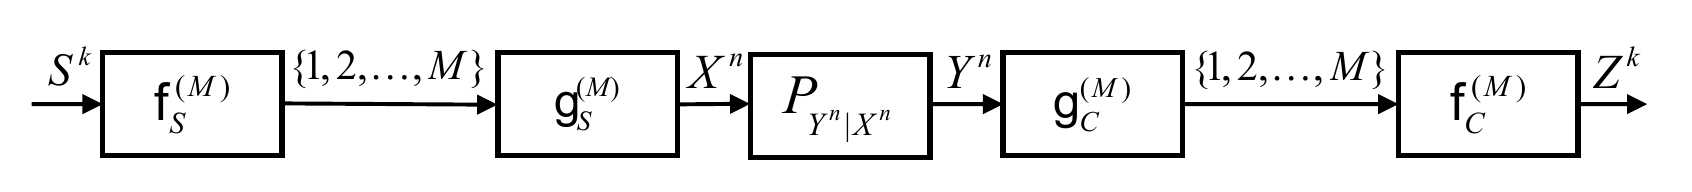
\includegraphics[width=0.85\linewidth]{fig/fig1.png}
\caption{원천 부호화와 채널 부호화의 구성.}
\end{figure}

최근 몇 년 사이 유한 부호 길이 정보이론은 원천 부호화, 채널 부호화, 결합 원천-채널 부호화(JSCC, joint source-channel coding)에 걸쳐 큰 관심을 받아 왔다. 원천-채널 부호화의 구성을 그림~1에 나타냈다. 원천 부호화, 곧 데이터 압축에서는 길이 $k$인 원천 출력 수열을 집합 $\{1,\dots,M\}$의 비트열로 사상한다. 그러면 수신 측에서 원천 기호를 정확히 복원하거나(거의 무손실 압축의 경우), 일정한 왜곡 충실도 안에서 복원할 수 있다(손실 압축의 경우). 이때 원천 알파벳 $\mathcal{S}$, 복원 알파벳 $\mathcal{Z}$, 왜곡 척도(distortion measure) $\dd:\mathcal{S}\times\mathcal{Z}\mapsto[0,+\infty]$가 주어진다. 원천 부호화의 유한 부호 길이 정보이론은 부호 길이 $k$, 오류 확률, 부호율 $\log M/k$라는 세 양 사이의 상충 관계(tradeoff)에 초점을 둔다 [10]. 여기서 오류 확률은 이산 원천 $S$에 대한 (거의) 무손실의 경우 $\P[S\neq Z]$ [9]이고, 손실의 경우 $\P[\dd(S,Z)>d]$이다. 채널 부호화의 기본 과제는 잡음이 있는 채널로 $M$개의 메시지를 부호 길이 $n$으로 전송하여, 수신 측이 $\epsilon$ 미만의 오류 확률로 메시지를 구별할 수 있게 하는 것이다 [11]. 이 경우 근본 문제는 부호 길이 $n$, 오류 요구 조건 $\epsilon$, 데이터율 $\log M/n$ 사이의 상충 관계를 규명하는 데 있다. 오늘날 대부분의 통신 시스템은 앞서 말한 원천 부호화와 채널 부호화를 차례로 수행하며, 이를 분리 원천-채널 부호화(SSCC, separate source-channel coding)라 한다. 그러나 이 구조는 유한 부호 길이에서 성능 손실이 크기 때문에, 원천과 채널의 부호기와 복호기를 함께 설계할 필요가 있다. 이런 JSCC 방식에서는 원천이 만든 길이 $k$인 수열을 채널 전송에 알맞은 길이 $n$인 수열로 직접 사상하므로, 데이터율은 $k/n$이 된다. 이때 $k$, $n$, 오류 확률 사이의 근본적인 상충 관계가 매우 중요하다 [12].

유한 부호 길이 영역에서는 위에서 말한 상충 관계를 해석적으로 정확히 기술하기 어렵다. 그래서 연구자들은 다음과 같은 촘촘하고(tight) 계산 가능한 달성 가능성 한계, 역 한계, 근사를 개발하는 쪽으로 방향을 돌린다.
\begin{itemize}
\item 달성 가능성 한계: 부호책 크기(code size) $M$, 부호 길이(원천 부호화에서는 $k$, 채널 부호화에서는 $n$), 오류 확률 $\epsilon$인 부호가 존재하면, 삼중쌍 $(M, k\ \text{또는}\ n, \epsilon)$을 달성 가능하다고 한다. 더 일반적으로 JSCC에서는 원천 입력 길이 $k$, 채널 부호 길이 $n$, 오류 확률 $\epsilon$인 결합 원천-채널 부호가 존재하면 삼중쌍 $(k,n,\epsilon)$이 달성 가능하다. 달성 가능성 한계는 달성 가능 영역의 내부 한계를 제공한다. 즉 매개변수 $(M, k\ \text{또는}\ n, \epsilon)$ 또는 $(k,n,\epsilon)$의 어떤 부분집합에 대해 부호가 존재함을 보장한다.
\item 역 한계: 역 한계는 비존재 결과를 제공한다. 즉 매개변수 $(M, k\ \text{또는}\ n, \epsilon)$ 또는 $(k,n,\epsilon)$의 특정 값에 대해서는 어떤 부호도 존재하지 않음을 보인다. 역 영역이 달성 가능 영역의 여집합과 일치하면 촘촘한 결과를 얻은 것이다. 다시 말해 가능한 가장 큰 영역을 결정한 것이다.
\item 근사: 많은 경우 영역을 촘촘하게 규명하는 일은 어떤 점근 영역에서만 가능하다(전형적인 영역은 $k$ 또는 $n\to\infty$이고 $\epsilon\to 0$인 경우이다). 그러나 $M$, $k$ 또는 $n$, $\epsilon$의 모든 비점근 값에 대해, 영역의 스케일링 법칙을 지배적인 항으로(상수 차이까지) 기술할 수 있는 경우가 흔하다. 또한 대수의 법칙과 에르고딕 정리 같은 도구를 쓰면, 원천 부호화에서는 주어진 $(M,k)$, 채널 부호화에서는 $(M,n)$, JSCC에서는 $(k,n)$에 대해 최적 부호의 오류 확률 $\epsilon$을 쉽게 계산할 수 있는 근사를 유도할 수 있다.
\end{itemize}

손실 원천 부호화의 유한 부호 길이 결과에 대한 최근 진전은 Zhou와 Motani의 단행본 [13]을 참고하면 된다. 이 책은 점대점(P2P)과 다중 단말 시나리오의 근본 한계를 모두 논의한다. 채널 부호화 쪽에서는 Polyanskiy, Poor, Verdú의 선구적 연구 [11]가 근본적인 비점근 한계를 확립했고, 이는 수많은 후속 연구를 이끌어 냈다. Kostina와 Verdú [14]는 손실 원천 부호화를 유한 부호 길이에서 포괄적으로 규명했으며, SSCC와 JSCC를 비교하는 데 귀중한 통찰을 주었다. 관련 연구는 이어지는 절에서 더 살펴본다. 이 논문에서 논의하는 주요 결과를 체계적으로 개관할 수 있도록 표~1에 정리했다. 이 유한 부호 길이 결과는 지연 제약이 엄격한 무선 통신 시스템의 근본 한계를 규명한다. 따라서 실제 무선 통신 방식을 평가하는 기준을 제공하고, 성능을 더 끌어올릴 여지가 있는 시나리오를 찾아 준다.

\begin{table}[t]
\centering
\caption{유한 부호 길이 영역의 주요 결과 요약}
\small
\renewcommand{\arraystretch}{1.35}
\begin{tabularx}{\linewidth}{|>{\centering\arraybackslash}m{0.13\linewidth}|>{\centering\arraybackslash}m{0.15\linewidth}|>{\centering\arraybackslash}m{0.22\linewidth}|>{\centering\arraybackslash}X|}
\hline
\textbf{분류} & \multicolumn{2}{c|}{\textbf{세부 분류 / 문제}} & \textbf{참고문헌} \\
\hline
\multirow{6}{=}{\centering 원천\\부호화} & \multicolumn{2}{c|}{P2P 무손실 압축} & [9, 15] \\
\cline{2-4}
 & \multirow{3}{=}{\centering P2P\\손실 압축} & 일반 무기억 원천 & [10, 16, 17, 18, 19, 20] \\
\cline{3-4}
 & & 가우스-마르코프 원천 & [21, 22, 23] \\
\cline{3-4}
 & & 불일치 & [24, 25] \\
\cline{2-4}
 & \multirow{2}{=}{\centering 다중 단말\\부호화} & Kaspi 문제 & [26, 27] \\
\cline{3-4}
 & & 점진적 정밀화 & [28, 29, 30, 31] \\
\hline
\multirow{3}{=}{\centering 채널\\부호화} & \multicolumn{2}{c|}{P2P} & [11, 32, 33, 34, 35, 36, 37, 38, 39, 40, 41, 42] \\
\cline{2-4}
 & \multicolumn{2}{c|}{다중 접속} & [43, 44, 45, 46, 47] \\
\cline{2-4}
 & \multicolumn{2}{c|}{대규모 접속} & [48, 49, 50, 51, 52, 53, 54] \\
\hline
\multirow{2}{=}{\centering JSCC} & \multicolumn{2}{c|}{이론} & [12, 55, 56, 57, 58, 59] \\
\cline{2-4}
 & \multicolumn{2}{c|}{응용} & [60, 61, 62] \\
\hline
\end{tabularx}
\end{table}

이 논문의 구성은 다음과 같다. 2장에서는 원천 부호화의 유한 부호 길이 한계를 검토한다. 2.1절에서는 이후 논의를 명확하고 일관되게 하기 위해 몇 가지 필수 용어를 정의한다. 이어서 2.2절, 2.3절, 2.4절에서 P2P 및 다중 단말 환경의 무손실 압축과 손실 압축을 다룬다. 3장에서는 채널 부호화의 유한 부호 길이 한계를 검토하며, 3.1절, 3.2절, 3.3절에서 각각 P2P 채널, 다중 접속 채널, 새로 떠오르는 대규모 접속 채널을 논의한다. 4장에서는 JSCC의 유한 부호 길이 한계를 검토한다. 5장에서는 유한 부호 길이 정보이론의 미해결 문제와 향후 연구 방향을 제시하고, 6장에서 논문을 맺는다.

\section{원천 부호화}

정보이론에서 원천 부호화는 데이터 압축이라고도 하며 [63], 크게 두 종류로 나뉜다. 바로 \emph{거의 무손실 압축}(almost lossless compression)과 \emph{손실 압축}이다. 거의 무손실 압축은 대개 이산 원천에 적용하며, 원래 정보를 모두 보존하여 완벽한 복원을 가능하게 한다. 손실 압축은 이산 원천과 연속 원천 모두에 적용한다. 손실 압축은 본질적이지 않은 정보를 버려 더 높은 효율을 얻고, 지정된 왜곡 수준 안에서 원래 데이터를 근사한다. 이 장에서는 P2P 환경의 무손실 압축과 손실 압축 각각에 대해 근본 한계의 진전을 검토한다. 그다음 다중 단말 환경의 근본 한계를 논의한다.

\subsection{기본 개념}

논의를 명확하고 표준적으로 하기 위해, 흔히 쓰는 용어와 정의 몇 가지를 소개한다. 고정 길이(fixed-length) 손실 압축에서는 알파벳이 $\mathcal{S}$이고 분포가 $P_S$인 일반 원천을, 복원 알파벳 $\mathcal{Z}$에서 뽑은 $M$개의 부호어(codeword) 가운데 하나로 사상한다. 손실 부호는 무작위화될 수도 있는 두 사상 $\ff:\mathcal{S}\mapsto\{1,\dots,M\}$과 $\gg:\{1,\dots,M\}\mapsto\mathcal{Z}$로 이루어진다. 이런 부호의 성능은 왜곡 척도 $\dd:\mathcal{S}\times\mathcal{Z}\mapsto[0,+\infty]$로 평가한다. 복호기 $\gg$가 주어지면, 최적 부호기는 각 원천 출력 $s$를 왜곡이 가장 작은 부호어에 할당한다. 즉 $\ff(s)=\arg\min_m \dd(s,\gg(m))$이다. 성능 지표로는 원천 통계에 대한 평균 왜곡을 흔히 쓴다. 이와 더불어, 지정된 왜곡 수준을 넘을 확률인 초과 왜곡 확률(excess-distortion probability)은 더 엄격한 평가 기준이 된다.

$\{\mathcal{S},\mathcal{Z},P_S,\dd\}$에 대한 $(M,d,\epsilon)$ 부호란 $|\ff|=M$이고 $\P[\dd(S,\gg(\ff(S)))>d]\le\epsilon$을 만족하는 부호이다. 왜곡 $d$와 초과 왜곡 확률 $\epsilon$에서 달성 가능한 최소 부호책 크기 $M^\star$는 다음과 같이 정의한다.
\begin{equation}
M^\star(d,\epsilon)\triangleq\min\{M:\exists(M,d,\epsilon)-\text{code}\}. \tag{1}
\end{equation}
특히 $d=0$이고 $\dd(s,z)=\mathbf{1}\{s\neq z\}$이면 거의 무손실 압축에 해당한다.

고정-고정(블록) 환경에서는 $\mathcal{S}^k$와 $\mathcal{Z}^k$가 각각 알파벳 $\mathcal{S}$와 $\mathcal{Z}$의 $k$겹 데카르트 곱이다. 이때 $\{\mathcal{S}^k,\mathcal{Z}^k,P_{S^k},\dd^k\}$에 대한 $(M,d,\epsilon)$ 부호를 $(k,M,d,\epsilon)$ 부호라 한다. $\epsilon$, $d$, 부호 길이 $k$를 고정할 때, 달성 가능한 최소 부호책 크기 $M^\star(k,d,\epsilon)$과 유한 부호 길이 율-왜곡 함수(rate-distortion function) $R^\star(k,d,\epsilon)$은 다음과 같이 정의한다.
\begin{equation}
M^\star(k,d,\epsilon)\triangleq\min\{M:\exists(k,M,d,\epsilon)-\text{code}\}, \tag{2}
\end{equation}
\begin{equation}
R^\star(k,d,\epsilon)\triangleq\frac{1}{k}\log M^\star(k,d,\epsilon). \tag{3}
\end{equation}

가변 길이(variable-length) 부호화에서 부호는 사상 $\ff:\mathcal{S}\mapsto\{0,1\}^*$과 $\gg:\{0,1\}^*\mapsto\mathcal{Z}$로 이루어진다. 여기서 $\{0,1\}^*$은 모든 이진 문자열의 집합이다. $\P[\dd(S,\gg(\ff(S)))\le d]=1$이면 이 부호가 왜곡 수준 $d$에서 동작한다고 한다. 왜곡 $d$에서 동작하는 부호 $(\ff,\gg)$에 대해, $s\in\mathcal{S}$에 할당된 이진 부호어의 길이를 $\ell(\ff(s))$, 곧 $\ff(s)$의 길이로 나타낸다.

\subsection{무손실 압축}

무손실 데이터 압축은 부호 길이가 고정되어 있는지에 따라 두 환경으로 나눌 수 있다. 하나는 \emph{거의 무손실 고정 길이 데이터 압축}이고, 다른 하나는 \emph{엄밀한 무손실 가변 길이 데이터 압축}이다 [9]. 가변 길이 무손실 압축은 접두(prefix) 사용 여부에 따라 다시 나뉜다. 고정-가변 부호의 성능은 평균 부호화 길이로 나타내는 것이 합리적이다. $R^\star(k,\epsilon)$은 최선의 부호의 압축률이 기호당 $R$비트를 넘을 확률을 $\epsilon$ 이하로 만드는 최소 율이다. 즉 다음을 만족하는 최소의 $R$이다.
\begin{equation}
\min_{\ff}\P[\ell(\ff(S^k))>kR]\le\epsilon. \tag{4}
\end{equation}
접두 부호화에서는 접두 조건(prefix condition) 아래에서 최소화해야 한다. 접두 부호화는 어떤 부호어도 다른 부호어의 접두가 되지 않도록 요구한다. 이 성질 덕분에, 고정-가변 길이로 부호화한 기호의 긴 흐름을 모호함 없이 구분하고 즉시 복호할 수 있다.\footnote{시작과 끝을 아는 단일 블록 압축에서는 접두 조건이 덜 중요하다.}

유한 부호 길이의 또 다른 근본 한계로, 달성 가능한 최선의 초과율 확률(excess-rate probability)을 나타내는 $\epsilon^\star(k,M)$이 있다.
\begin{equation}
\epsilon^\star(k,M)\triangleq\min_{\ff}\P[\ell(\ff(S^k))\ge\log M]. \tag{5}
\end{equation}
여기서 오류 사건은 압축된 부호어의 길이가 $\log M$을 넘을 때 일어나며, $M$은 압축기가 내놓는 서로 다른 출력의 개수이다. Verdú [64]와 Kontoyiannis 등 [9]는 접두 제약이 없는 엄밀한 무손실 가변 길이 부호의 근본 한계 $\epsilon^\star(k,M)$이 고정 길이 거의 무손실 부호의 최소 오류 확률과 같음을 보였다. 이 결과는 $M<|\mathcal{S}|^k$인 비자명한 압축의 경우와 자명한 경우 모두에서 성립한다. 자명한 경우는 간결함을 위해 생략한다. 비자명한 경우, 최적 고정-고정 압축기는 $\mathcal{S}^k$에서 확률이 가장 큰 $M-1$개의 원소 각각에 길이 $\log M$인 고유한 이진 문자열을 할당한다. 그리고 나머지 원소는 모두 길이 $\log M$인 또 다른 이진 문자열 하나에 할당하는데, 이 문자열은 부호화 실패를 뜻한다. 최적 부호가 $\log M$보다 짧은 길이로 부호화한 문자열만 오류 없이 복호할 수 있다.

\subsubsection{비점근 한계}

앞에서는 부호 길이 $k$를 포함하는 수열 표기를 썼다. 일반적인 비점근 한계를 제시할 때는 명확하고 간결하게 하기 위해 [14, 65]처럼 단일 시행(single-shot) 표기를 쓴다. 구체적으로, 확률변수 $S$와 그 실현값 $s$는 길이 $k$인 수열 전체를 나타낼 수 있는 추상적인 기호이다. 수열을 나타낼 때는 해당 알파벳 $\mathcal{S}$를 단일 문자(single-letter) 알파벳의 $k$겹 데카르트 곱으로 해석해야 한다.

분포가 $P_S$인 무작위 원천 출력 $S$의 정보는 [9, eq.~(3)]에 따라 다음과 같이 정의한다.
\begin{equation}
\iinf_S(s)=\log\frac{1}{P_S(s)}. \tag{6}
\end{equation}
$\ff^\star$를 최적 압축기라 하면, 최적 부호 길이 $\ell(\ff^\star(S))$의 분포는 $\iinf_S(S)$의 분포와 밀접하게 연결되어 있다. 그뿐 아니라, 이와 비슷한 정보 확률변수(information random variable)가 비점근 정보이론의 근본 한계를 얻는 데 결정적인 역할을 한다는 점에도 주목해야 한다.

\paragraph{1) 달성 가능성 한계}
최선의 부호에 대한 달성 가능성 한계를 분석하는 주된 방법은 두 가지이다. 하나는 (6)에서 정의한 정보 확률변수 $\iinf_S(S)$를 분석하여 최적 부호기가 만드는 부호 길이의 한계를 얻는 방법이다. 다른 하나는 무작위 비닝(random binning)을 정확히 분석하여 최적 부호의 성능에 대한 하한을 유도하는 방법이다. 알파벳이 유한하거나 가산 무한인 임의의 원천에 대해, 간단하면서도 강력한 달성 가능성 한계가 있다. 최적 부호기가 만드는 부호 길이는 원천 고유의 정보를 넘지 않는다는 것이다. 다시 말해 $\ell(\ff^\star(S))$의 분포 함수는 $\iinf_S(S)$의 분포 함수를 지배한다. [15]는 이 결과를 더 정밀하게 다듬어 두 양의 꼬리 확률을 한정했다. 즉 $\P[\ell(\ff^\star(S))\ge a]\le\P[\iinf_S(S)\ge a]$이다. 이 관찰은 $\mathcal{S}$의 원소를 확률이 증가하지 않는 순서로 늘어놓는 데서 나온다. 이렇게 늘어놓으면 각 원소의 확률은 그 원소의 순위의 역수를 넘지 않는다. 채널 부호화의 무작위 부호화(random coding) [11]와 비슷하게, 유한 부호 길이에서 달성 가능한 오류 확률을 얻는 한 방법이 [9]의 \emph{무작위 비닝}이다. [10] 같은 손실 압축 연구에서는 \emph{무작위 부호화}라는 용어를 그대로 썼다. 이 설정에서는 압축기가 더 이상 단사 사상일 필요가 없다. 복원기는 둘 이상의 원천 실현값으로 설명될 수 있는 레이블을 받으면 그중 가장 그럴듯한 것을 고르며, 동률이면 임의로 고른다. 다만 이 접근은 특히 부호 길이가 클 때 새로운 계산상의 어려움을 낳는다.

\paragraph{2) 역 한계}
일부 연구는 정보 확률변수에 기반하여 역 한계를 유도한다. 이 역 한계는 최적 부호기 $\ff^\star$가 출력하는 부호어 길이에 관한 것이다. Verdú [15]는 $\ell(\ff^\star(S))$에 대한 역 한계 $\max_{\tau>0}\bigl[\P[\iinf_S(S)\ge\log M+\tau]-2^{-\tau}\bigr]\le\P[\ell(\ff^\star(S))\ge\log M]$을 제시했다. 이 한계는 고정된 임의의 $\tau>0$에 대해 원천 알파벳의 부분집합 $\mathcal{L}=\{i\in\mathcal{S}:P_S(i)\le 2^{-\tau}M^{-1}\}$을 고려하여 얻었다. 이후 Kontoyiannis 등 [9]는 임의의 압축기의 부호 길이 $\ell(\ff(S))$를 정보 확률변수 $\iinf_S(S)$와 비교했다. 이 결과는 점별(pointwise) 점근 결과를 크게 진전시켰고, 이를 바탕으로 원천 $\{P_{S^k}\}_{k=1}^\infty$의 원천 분산도(source dispersion) $\limsup_{k\to\infty}\frac{1}{k}\Var[\ell(\ff_k^\star(S^k))]$가 그 원천의 바렌트로피(varentropy, 최소 부호화 분산) $\Var[\iinf_S(S)]$와 같다는 결론으로 이어졌다.

정보 확률변수에 기반한 방법은 비점근 한계를 얻는 데 널리 쓰여 왔지만, 언제나 촘촘한 한계를 주지는 않는다 [9, Fig.~1]. 이 때문에 다른 접근법이 개발되었다. 앞서 달성 가능성 한계에서 소개한 무작위 부호화 [9, 10]와, 최선의 손실 압축 부호에 대한 역 한계를 유도할 때 쓰는 가설 검정 [10]이 그 예이다.

\subsubsection{근사}

접두 가변 길이 부호에 대해서는 최소 평균 압축률 $\bar{R}(k)$의 점근적 거동이 널리 알려진 결과로 [66]에 주어져 있다. 여기서 `평균'은 모든 압축기의 전체적인 성능을 가리키므로, 이 율은 초과율 확률과 무관하다. Kontoyiannis [67]는 이후 임의의 접두 부호의 길이에 대해 다른 종류의 가우스 근사(Gaussian approximation)를 제시했다. 구체적으로, Kontoyiannis는 먼저 $\ell(\ff(S))$를 근사적으로 가우스 분포를 따르는 확률변수로 한정하고, 이어서 이 한계를 반복 로그 법칙(LIL, law of the iterated logarithm) 수준으로 정밀화했다. 부호 길이 분포의 대편차(large deviations)에 대해 Merhav [68]는 기억이 있는 일부 원천에서 대편차 분석에 기반한 최적 오류 지수(error exponent)가 접두 제약과 압축기의 보편성(universality) 때문에 낮아지지 않음을 보였다. Lempel-Ziv 압축기는 그 지수를 달성한다 [69]. 이어서 Kontoyiannis [9, Sec.~III]는 최소 평균 압축률의 점근적 거동을 엔트로피율 $H(S)$로 완전히 기술했다.

최적의 거의 무손실 고정-고정 부호와 최적의 엄밀한 무손실 고정-가변 부호는 밀접하게 대응한다. 이 대응에 근거하여, 다음 연구들은 두 환경 모두에 적용된다. 점근 영역에서 Csiszár 등 [70]은 오류 확률의 지수적 감소를 매개변수화했다. Szpankowski 등 [71]은 등확률이 아닌 원천에 대해 최소 평균 압축률의 근사를 제시했다. [66]의 접두 부호와 달리, $\bar{R}(k)$의 근사에서 추가 2차 항(second-order term) $-\frac{2}{k}\log k$를 얻었다. 이 결과는 이후 $\iinf_S(S)$가 비격자(non-lattice)인 경우로 확장되었다.\footnote{이산 확률변수의 모든 확률 질량이 어떤 격자 $\{\nu+n\zeta\}$ ($n\in\mathbb{Z}$)의 부분집합 위에 놓이면, 그 확률변수를 격자형(lattice)이라 한다.} 한편 달성 가능한 최소 원천 부호율 $R^\star(k,\epsilon)$에 대해서는 Yushkevich [72]가 근사를 유도했다. Strassen [73]은 이 결과를 $\iinf_S(S)$가 비격자인 등확률이 아닌 무기억 원천(memoryless source)으로 확장했다. Kontoyiannis [9]는 $R^\star(k,\epsilon)$의 근사에 대한 Strassen의 완전한 증명에 논란의 여지가 있다고 지적하고, 다음 식과 그에 대한 상세한 증명을 제시했다.
\begin{equation}
R^\star(k,\epsilon)=H(S)+\sqrt{\frac{V(S)}{k}}\,Q^{-1}(\epsilon)-\frac{1}{2k}\log k+O\!\left(\frac{1}{k}\right). \tag{7}
\end{equation}
두 핵심 양은 $H(S)=\E[\iinf_S(S)]$와 $V(S)=\Var[\iinf_S(S)]$로 정의한다. $Q^{-1}(\cdot)$은 표준 가우스 분포의 상보 누적 분포 함수(CDF, cumulative distribution function)의 역함수이다. 직관적으로 보면, 중심극한정리(CLT, central limit theorem)에 의해 $\iinf_{S^k}(S^k)=\sum_{i=1}^k\iinf_S(S_i)$의 분포가 근사적으로 가우스 분포이기 때문에 이런 결과가 나온다. 여기서 $S^k$는 길이 $k$인 원천 출력 수열이다. 이 결과는 정밀한 역 한계와 달성 가능성 한계에 고전적인 Berry-Esséen 한계 [74]를 함께 적용해 얻는다.
